\documentclass[t]{beamer}
   \usepackage{bm,amssymb, amsmath, graphicx}
   \usepackage{booktabs}
   \usepackage{caption}
\usepackage{subcaption}
\usepackage{float}
\usepackage{mathrsfs}
\usepackage{array} 
\usepackage{rotating}
 \providecommand{\abs}[1]{\lvert#1\rvert}
\providecommand{\norm}[1]{\lVert#1\rVert}
 \usetheme{Boadilla}
 \usefonttheme[onlymath]{serif}
 \setbeamertemplate{blocks}[rounded][shadow=false]
 \setbeamertemplate{navigation symbols}{}


 \title[The Joint Graphical Lasso]{Joint Estimation of Graphical Models \\ Across Multiple Classes}
 % \subtitle{P. Danaher, P. Wang \& D. Witten}
 \author[Abrahamsen, Bai, Rahman \& Skripnikov]{Tavis Abrahamsen, Ray Bai, \\ Syed Rahman, Andrey Skripnikov}
 \institute[ ]{Department of Statistics \\ University of Florida}
\date{April 22, 2015}
\begin{document}



\begin{frame}
 \titlepage
\end{frame}

\begin{frame}
\frametitle{Background}
Suppose that observations $\bm{x}_{1},\bm{x}_{2},\ldots,\bm{x}_{n} \in \mathbb{R}^{P}$ are independent and identically distributed $N(\bm{\mu},\bm{\Sigma})$ where $\bm{\mu} \in \mathbb{R}^{p}$ and $\bm{\Sigma}$ is a positive definite $p\times p$ matrix. 

\bigskip
\pause
The zeros in the inverse covariance matrix $\bm{\Sigma}^{-1}$ correspond to pairs of features that are conditionally independent - that is, pairs of variables that are independent of each other, given all the other variables in the data set.

\bigskip
\pause
In a Gaussian graphical model, the conditional dependence relationships are represented by a graph in which nodes represent the features and edges connect conditionally dependent pairs of features.
\end{frame}


\begin{frame}
\frametitle{Background}
A natural way to estimate the precision (or concentration) matrix $\bm{\Sigma}^{-1}$ is via maximum likelihood.  Letting $\bm{S}$ denote the empirical covariance matrix of $X$, the Gaussian log likelihood takes the form (up to a constant)
\small
\begin{equation*}
\frac{n}{2}\log\, \det \bm{\Sigma}^{-1} - \mbox{trace}\left(\bm{S\,\Sigma}^{-1}\right)
\end{equation*}

\normalsize
\bigskip
\pause
Maximizing this function with respect to $\bm{\Sigma}^{-1}$ yields the maximum likelihood estimate $S^{-1}$.

\bigskip
\pause
Problems with using the MLE of $\bm{\Sigma}^{-1}$:
\begin{itemize}
	\item[1.] In the high dimensional setting where $p > n$ the matrix $\bm{S}$ is singular and cannot be inverted to yield an estimate of $\bm{\Sigma}^{-1}$.
	
	\bigskip
	\item[2.] Even when $\bm{S}^{-1}$ exists, this estimator will typically not be sparse.
\end{itemize}
\end{frame}

\begin{frame}
\frametitle{Background}
One method for obtaining sparse estimates of $\bm{\Sigma}^{-1}$ is to instead solve the \textit{graphical lasso} problem
\small
\begin{equation*}
\max_{\bm{\Theta}} \log\,\det \bm{\Theta} - \mbox{trace}\left(\bm{S \,\Theta}\right) - \lambda ||\bm{\Theta}||_{1},
\end{equation*}
\normalsize
where $\lambda$ is a nonnegative tuning parameter. 



\bigskip
\pause
Advantages of using the graphical lasso estimator:
\begin{itemize}
\item[1.]  The $l_{1}$ penalty term yields sparse estimates of $\bm{\Sigma^{-1}}$ when $\lambda$ is ``large".

\bigskip
\item[2.] This problem can be solved even if $p \gg n$.
\end{itemize}
\end{frame}


\begin{frame}
\frametitle{Estimating Models for Heterogeneous Data}
\textbf{Problem}: The standard formulation for estimating a Gaussian graphical model assumes that each observation is drawn from the same distribution. However, in many datasets the observations may correspond to several distinct classes. 

\bigskip
\pause
Estimating a single graphical model would mask the underlying heterogeneity, while estimating separate models for each category ignores the common structure.

\bigskip
\pause
We want to \textbf{jointly} estimate several graphical models corresponding to different categories. In this presentation, we will describe three algorithms that enable us to do this.

\end{frame}


\begin{frame}
\frametitle{Motivation - Genetics}
Graphical models are of particular interest in the analysis of gene expression data since they can provide a useful tool for visualizing the relationships among genes and generating biological hypotheses. 

\bigskip
\pause
The datasets may correspond to several distinct classes. For example, suppose a cancer researcher collects gene expression measurements for a set of cancer tissue samples and a set of normal tissue samples.  One might want to estimate a graphical model for the cancer samples and a graphical model for the normal samples.

\bigskip
\pause
One might expect the two graphical models to be similar to each other since both are based on the same type of tissue, but also have important differences resulting from the fact that gene networks are often dysregulated in cancer. 

\end{frame}

  \begin{frame}
\frametitle{Problem Formulation}
  
 
  Suppose we have a heterogeneous data set with $p$ variables and $K$ categories.
  
\bigskip
\pause
   The $k$-th
  category contains $n_k$ observations $(\boldsymbol{x}_1^{(k)},...,\boldsymbol{x}_{n_k}^{(k)})$, where each $\boldsymbol{x}_i^{(k)} = (x_{i,1}^{(k)},...,x_{i,p}^{(k)})$ is a $p$-dimensional row vector.
\bigskip
\pause

   Without loss of generality, we assume the observations in the same category are centered along each variable, i.e., $\sum_{i=1}^{n_k} x_{i,j}^{(k)} = 0$ for all $1 \leq j \leq p$ and $1 \leq k \leq K$.
 
  \end{frame}
  


  \begin{frame}{Problem Formulation}
  
   We further assume that $\boldsymbol{x}_1^{(k)},...,\boldsymbol{x}_{n_k}^{(k)}$ are independent and identically distributed, sampled
    from a $p$-variate Gaussian distribution with mean zero (without loss of generality since we
    center the data) and covariance matrix $\Sigma^{(k)}$. 
    
    \
    
     Let $\Omega^{(k)} = (\Sigma^{(k)})^{-1} = (\omega_{j,j'}^{(k)})_{pxp}$.
     
\bigskip
\pause
     
     Then the likelihood function for $k$-th category will look like this:
 
 
  \begin{equation*} l(\Omega^{(k)}) = -\frac{n_k}{2} \log(2\pi) + \frac{n_k}{2}[ \log\{ \det(\Omega^{(k)})\} - \mbox{trace}(\hat{\Sigma}^{(k)} \Omega^{(k)})], \end{equation*}
   
  
   where $\hat{\Sigma}^{(k)}$ is the sample covariance matrix for the k-th category.
   
   \end{frame}
   
   \begin{frame}{Problem Formulation}
   The most direct way to deal with such heterogeneous data is to estimate $K$ individual
    graphical models. We can compute a separate $l_1$-regularized estimator for each category $k$,
   $ 1 \leq k \leq K$, by solving
   

\begin{equation*}
     \underset{\Omega^{(k)}}{\mbox{min}} \  \mbox{trace} (\hat{\Sigma}^{(k)} \Omega^{(k)}) - \log\{ \det(\Omega^{(k)})\} + \lambda_k \sum_{j \neq j'} |\omega_{j,j'}^{(k)}|,
\end{equation*}
    
    \
     
     where the minimum is taken over symmetric positive definite matrices.
     
     \bigskip
\pause
     
 This problem can be efficiently solved by existing algorithms such as $glasso$ of Freidman et al. (2008). However, we would prefer to jointly estimate several graphical models instead of estimating each one separately.
       
   \end{frame}
   
    \begin{frame}{Joint Estimation}
      
      To improve estimation in cases where graphical models for different categories may share
      some common structure, J. Guo, E. Levina, G. Michailidis, and J. Zhu propose the following \textit{joint estimation method} in their paper ``Joint Estimation of Multiple Graphical Models'' (2009).
      
      \bigskip
\pause
      
       First, they reparameterize each $\omega_{j,j'}^{(k)}$  as
      
      \begin{equation*}
     \omega_{j,j'}^{(k)} = \theta_{j,j'} \gamma_{j,j'}^{(k)}, 1\leq j \neq j' \leq p, \ 1\leq k \leq K 
\end{equation*}.

      \bigskip
\pause
      For identifiability purposes, we restrict $\theta_{j,j'} > 0, \ 1\leq j \neq j' \leq p$. To preserve symmetry, they also require $\theta_{j,j'} = \theta_{j',j}$ and $\gamma_{j,j'}^{(k)} = \gamma_{j',j}^{(k)}$, $1 \leq j \neq j' \leq p$ and $1 \leq k \leq K$.
      
      \bigskip
\pause
      
       This decomposition treats $\{ \omega_{j,j'}^{(1)},...,\omega_{j,j'}^{(K)} \}$ as a group, with the common factor $\theta_{j,j'}$ controlling the presence of the link between nodes $j$ and $j'$ in any of the categories, and $\gamma_{j,j'}^{(k)}$ reflects the differences between categories. 
      
      \end{frame}


      \begin{frame}{Joint Estimation}
      
        
        
        Let $\Theta = (\theta_{j,j'})_{pxp}$ and $\Gamma^{(k)} = (\gamma_{j,j'}^{(k)})_{pxp}$. To estimate this model, we propose the following penalized criterion:
        
        \
        \begin{equation}
        \underset{\Theta,\{ \Gamma^{(k)}\}_{k=1}^{K}}{\min}   \sum_{k=1}^{K} [\mbox{trace}(\hat{\Sigma} \Omega^{(k)}) - \log\{ \det(\Omega^{(k)})\}] \ +  \eta_1 \underset{j \neq j'}{\sum} \theta_{j,j'} +   
        \eta_2 \underset{j \neq j'}{\sum} \sum_{k=1}^K |\gamma_{j,j'}^{(k)}|,
        \end{equation}
        \
        
        subject to    $ \ \ \omega_{j,j'}^{(k)}=\theta_{j,j'} \gamma_{j,j'}^{(k)}$, $\theta_{j,j'} > 0$, $1 \leq j,j' \leq p$
        
        $\ \ \ \ \ \ \ \ \ \ \ \ \ \ \ \ \theta_{j,j'} = \theta_{j',j}$, $\gamma_{j,j'}^{(k)} = \gamma_{j',j}^{(k)}, 1 \leq j \neq j' \leq p$; $1 \leq k \leq K$
        
        $\ \ \ \ \ \ \ \ \ \ \ \ \  \ \ \ \theta_{j,j'}=1,\gamma_{j,j}^{(k)}=\omega_{j,j'}^{(k)} , 1 \leq j \leq p$; $1 \leq k \leq K$,
        
        \
        
        where $\eta_1$ and $\eta_2$ are two tuning parameters.
        
        
      \end{frame}
   
    \begin{frame}{Joint Estimation}
    
   \begin{itemize}

    \item{ The first parameter, $\eta_1$ , controls the sparsity of
      the common factors $\theta_{j,j'}$ and it can effectively remove the common zero elements across
      $\Omega^{(1)},...,\Omega^{(K)}$; i.e., if $\theta_{j,j'}$ is shrunk to zero, there will be no link between nodes $j$ and $j'$ in
      any of the K graphs.}
      \pause
      \item{ If $\theta_{j,j'}$ is not zero, some of the $\gamma_{j,j'}^{(k)}$’s (and hence some of the $\omega_{j,j'}^{(k)}$ ’s) can
      still be set to zero by the second penalty controlled by $\eta_2$. This allows graphs belonging to different categories
      to have different structures.}
    
    \end{itemize}  
      
    \end{frame}

    \begin{frame}{Joint Estimation}
    
    To simplify the model, the two tuning parameters $\eta_1$ and $\eta_2$ in (1) can be replaced by a
      single tuning parameter, by letting $\eta = \eta_1 \eta_2$. It turns out that solving (1) is equivalent to
      solving
      
      \begin{equation}  
      \underset{\Theta,\{ \Gamma^{(k)}\}_{k=1}^{K}}{\min}   \sum_{k=1}^{K} [\mbox{trace}(\hat{\Sigma} \Omega^{(k)}) - \log\{ \det(\Omega^{(k)})\}] +  \underset{j \neq j'}{\sum} \theta_{j,j'} + \eta \underset{j \neq j'}{\sum} \sum_{k=1}^K |\gamma_{j,j'}^{(k)}|,   
       \end{equation}
       
        \
        
        subject to    $\ \ \omega_{j,j'}^{(k)}=\theta_{j,j'} \gamma_{j,j'}^{(k)}$, $\theta_{j,j'} > 0$, $1 \leq j,j' \leq p$
        
        $\ \ \ \ \ \ \ \ \ \ \ \ \ \ \ \ \theta_{j,j'} = \theta_{j',j}$, $\gamma_{j,j'}^{(k)} = \gamma_{j',j}^{(k)}, 1 \leq j \neq j' \leq p$; $1 \leq k \leq K$
        
        $\ \ \ \ \ \ \ \ \ \ \ \ \ \  \ \ \theta_{j,j'}=1,\gamma_{j,j}^{(k)}=\omega_{j,j'}^{(k)} , 1 \leq j \leq p$; $1 \leq k \leq K$,
        
        \
        \end{frame}
        
 
           \begin{frame}{Joint Estimation}
            
            
             First, Guo et al. reformulate the problem (2) in a more convenient form for computational purposes. 

\bigskip
\pause
 Let $\{ \hat{\Omega}^{(k)}\}_{k=1}^K$ be a local minimizer of
              
              
             \begin{equation}
              \underset{ \{ \Omega^{(k)}\}_{k=1}^{K}}{\min}   \sum_{k=1}^{K} [\mbox{trace}(\hat{\Sigma} \Omega^{(k)}) - \log\{ \det(\Omega^{(k)})\}] + \lambda \underset{j \neq j'}{\sum} \sqrt{\sum_{k=1}^K |\omega_{j,j'}^{(k)}|},
              \end{equation}
              \
              
              where $\lambda = 2 \sqrt{\eta}$. Then, there exists a local minimizer of (2), $(\hat{\Theta}, \{ \hat{\Gamma}\}_{k=1}^K) $, such that $\hat{\Omega}^{(k)} = \hat{\Theta}^{(k)} \hat{\Gamma}^{(k)}$, for all $1 \leq k \leq K$. On the other hand, if $(\hat{\Theta},\{ \hat{\Gamma}^{(k)}\}_{k=1}^K)$ is a local minimizer of $(2)$, then there also exists a local minimizer of $(3)$, $\{ \hat{\Omega}^{(k)}\}_{k=1}^K$, such that $\hat{\Omega}^{(k)} = \hat{\Theta}^{(k)} \hat{\Gamma}^{(k)}$ for all $1 \leq k \leq K$.
              
             \end{frame}

              \begin{frame}{Joint Estimation}
               One can see that because of the penalty term in $(3)$, the optimization criterion is \textit{not} convex.   
               \bigskip


               \pause
                In order to reach convexity, an iterative optimization approach based on local linear approximation (LLA) is used (Zou and Li, 2008). If $p_{\lambda}(|\omega|)$ denotes the penalty term then LLA does the following:
                        
                        \begin{equation*}p_{\lambda}(|\omega|) \approx p_{\lambda}(|\omega^0|) + p'_{\lambda}(|\omega^0|)(|\omega| - |\omega^0|), \mbox{ for } \omega \approx \omega^0. 
\end{equation*} 
                     
 \pause
                         Specifically, letting $(\omega^{(k)}_{j,j'})^{(t)}$
                   denote
                  the estimates from the previous iteration $t$, we approximate
            \begin{equation*}      
                 \sqrt{\sum_{k=1}^K |\omega_{j,j'}^{(k)}|} \sim \frac{\sum_{k=1}^K |\omega_{j,j'}^{(k)}|}{\sqrt{\sum_{k=1}^K |(\omega_{j,j'}^{(k)})^{(t)}|}}. 
\end{equation*}
                 \bigskip
\pause
                 
                  LLA estimate helps alleviate the computation burden 
                 and overcome the potential local minima problem in minimizing the nonconvex
                 function.
                
                
                 \end{frame}
                 
  
          \begin{frame}{Joint Estimation Algorithm}
             
             Thus, at the $(t+1)$-th iteration of our joint estimation algorithm, problem (3) may be decomposed into K individual optimization
             problems:
             
             
             \begin{equation}
             (\Omega^{(k)})^{(t+1)} = \arg \underset{\Omega^{(k)}}{\min} \ \mbox{trace}(\hat{\Sigma}^{(k)}  \Omega^{(k)}) - \log\{ \det(\Omega^{(k)})\} + \lambda \sum_{j \neq j'} \tau_{j,j'}^{(k)} |\omega_{j,j'}^{(k)}|,
             \end{equation}
             
             where $\tau_{j,j'}^{(k)} = (\sum_{k=1}^K |(\omega_{j,j'}^{(k)})^{(t)}|)^{-1/2}$.
             
             \bigskip
             \pause
              Note that criterion (4) is exactly the sparse precision
             matrix estimation problem with weighted $l_1$ penalty; the solution can be efficiently computed
             using $glasso$.
            
            
            \end{frame} 
            
            
             \begin{frame}{Convexity of the Criterion}
              
                \begin{itemize}
\item
                $\mbox{trace}(\hat{\Sigma}^{(k)}  \Omega^{(k)})$ is an affine function of elements of $\Omega^{(k)}$, therefore is convex.
                
                \pause
                \item
                $\log\{ \det(\Omega^{(k)})\}$ is convex by the restriction to the line proof from class.
                
                \pause
                \item
                $\lambda \sum_{j \neq j'} \tau_{j,j'}^{(k)} |\omega_{j,j'}^{(k)}|$ is convex as an affine function of elements of $\Omega^{(k)}$.
               \end{itemize}
               \bigskip

                The sum of convex functions is convex, therefore the minimization criterion is a convex function of $\Omega^{(k)}$.
                
               \end{frame}
               
               \begin{frame}{Joint Estimation Algorithm}  
                   In summary, the proposed algorithm for solving            
\begin{equation*}
              \underset{ \{ \Omega^{(k)}\}_{k=1}^{K}}{\min}   \sum_{k=1}^{K} [\mbox{trace}(\hat{\Sigma} \Omega^{(k)}) - \log\{ \det(\Omega^{(k)})\}] + \lambda \underset{j \neq j'}{\sum} \sqrt{\sum_{k=1}^K |\omega_{j,j'}^{(k)}|},
              \end{equation*}
              \ is:
                   \pause
                   \
                  \begin{enumerate}[(a)]
\item
                 Initialize $\hat{\Omega}^{(k)}=(\hat{\Sigma}^{(k)} + \nu I_p)^{-1}$ for all $1 \leq k \leq K$, where $I_p$ is the identity matrix and the constant $\nu$ is chosen to guarantee $\hat{\Sigma}^{(k)} + \nu I_p$ is positive definite;
                  
                  \item
                        Using $glasso$, update $\hat{\Omega}^{(k)}$ by (4) for all $1 \leq k \leq K$.
                  
                  \item
                  
                  Repeat the previous step until convergence is achieved.
                 \end{enumerate}
                
                \end{frame}
                
                
           \begin{frame}{Model Selection.}
            
              The tuning parameter $\lambda$ in $(4)$ controls the sparsity of the resulting estimator. 
\bigskip
\pause

Guo et al. select the optimal tuning parameter by minimizing a Bayesian information criterion (BIC), which
              balances the goodness of fit and the model complexity. Specifically, we define BIC for the
              proposed joint estimation method as
              \begin{equation*}
               BIC(\lambda) = \sum_{k=1}^K [\mbox{trace}(\hat{\Sigma}^{(k)} \hat{\Omega}_{\lambda}^{(k)}) - \log \{ \det(\hat{\Omega}_{\lambda}^{(k)} \} + \log(n_k) df_k] 
              \end{equation*}
              
              where $\hat{\Omega}_{\lambda}^{(1)},...,\hat{\Omega}_{\lambda}^{(K)}$ are the estimates from (4) with tuning parameter $\lambda$ and the degrees of
              freedom are  $df_k =  \# \{ (j,j') : j<j', \hat{\omega}_{j,j'}^{(k)} \neq 0 \}.$
              
              \end{frame}

\begin{frame}
\frametitle{Simulation Study}
To assess the performance of the joint estimation algorithm in Guo et al., three types of simulated networks are simulated: a chain network, a 5-nearest neighbors network, and a scale-free (power law) network. In all cases, $p = 100$ features and $K = 3$. For $k = 1, ..., K$, $n_k = 100$ iid observations from a multiariate normal distribution $N(\bm{0}, (\bm{\Omega}^{(k)})^{-1})$, where $\bm{\Omega}^{(k)}$ is the precision matrix for the $k$-th category.
\bigskip
\pause

A constant $\rho$ is used to add heterogeneity to the common structure by creating additional indiivdual links (i.e. $\rho$ is the ratio of the number of individual links to the number of common links).

\end{frame}

\begin{frame}
\frametitle{Networks}
\centering
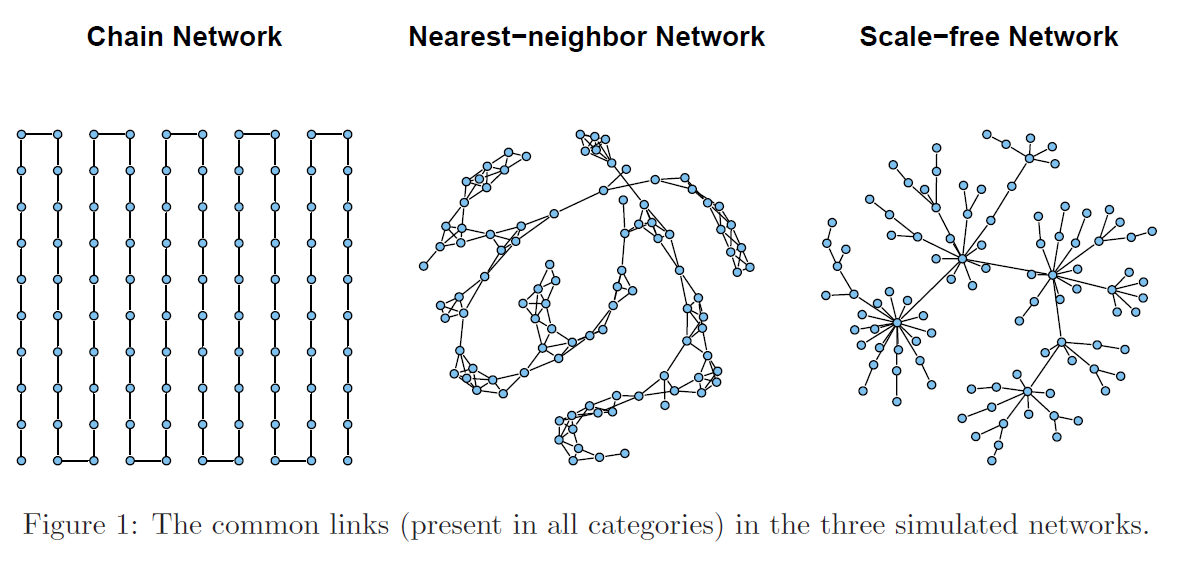
\includegraphics[height=2in]{networks.png}
\end{frame}

\begin{frame}
\frametitle{Model Diagnostics}
We compare the \textit{joint estimation method} to the \textit{separate estimation method}. To assess performance:
\begin{itemize}
\item
\pause
Plot ROC curves which plot the average proportion of correctly detected links against the average false positive range of values over a range of values of $\lambda$. 
\item
\pause
Compute and compare the following metrics: average entropy loss (EL), average Frobenius loss (FL), average false positive (FP) and average false negative (FN) rates, and the average rate of mis-identified common zeros among the categories (CZ).
\end{itemize}
\end{frame}


\begin{frame}
\frametitle{Simulation Results}
\centering
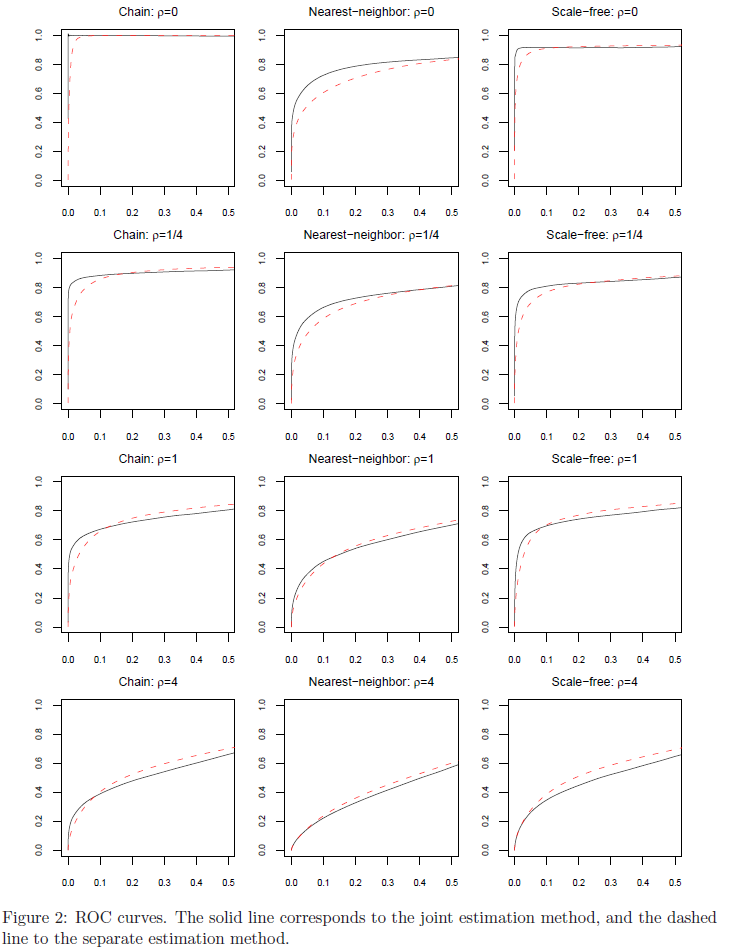
\includegraphics[height=3in]{guocurves.png}
\end{frame}


\begin{frame}
\frametitle{Simulation Results}
\centering
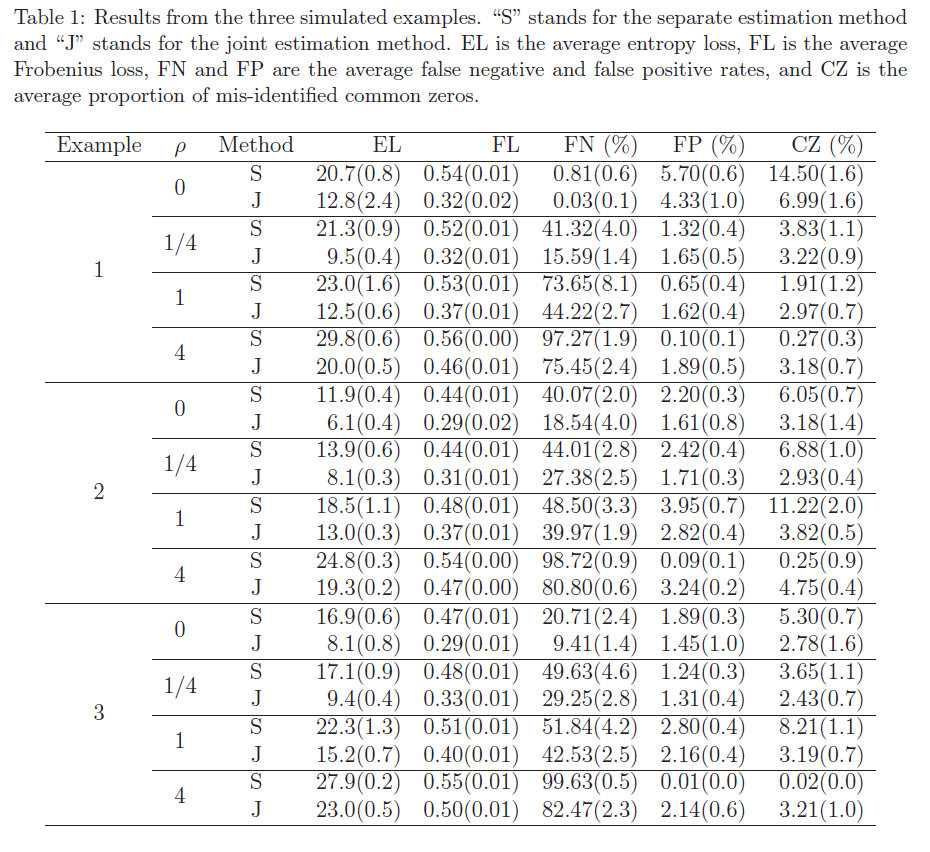
\includegraphics[height=3in]{guoresults.png}
\end{frame}

\begin{frame}
\frametitle{Simulation Results}
As the estimated ROC curves in Figure 2 show, the joint estimation method dominates the separate estimation method when the proportion of individual links is low. When the proportion of indvidual links is \textit{high}, the methods perform similarly.
\bigskip
\pause

As Table 1 shows, the joint estimation method produces lower entropy and Frobenius losses, as well as lower false negative rates.
\bigskip
\pause 

When the proportion of common links is high enough, it produces lower false positive rates and performs better at identifying common zeros than the separate estimation method.

\bigskip
\pause
\textbf{Conclusion}: In the presence of a common structure, the joint estimation method outperforms the separate estimation method. In the absence of a common structure, their performance is fairly similar.
\end{frame}
\begin{frame}
\frametitle{Data Example}
Webpages from websites at computer science departments in four universities (Cornell, Texas, Washington, and Wisconsin) are manually classified into seven categories: student, faculty, staff, department, course, project, and other. The joint estimation method is applied to $n = 1396$ documents in the four largest categories and $p = 100$ terms, and links between the terms are explored. The resulting common structure is shown in Figure 3.
\bigskip
\pause

The model also allows us to explore the heterogeneity between different categories. For example, the graphs for the ``student'' and ``faculty'' categories have some links that appear in only one or the other (e.g. the terms ``teach'' and ``assist'' are only linked in the ``student'' category, while ``assist-professor'' and ``select-public'' are only linked in the ``faculty'' category.
\end{frame}


\begin{frame}
\frametitle{Data Example}
\centering
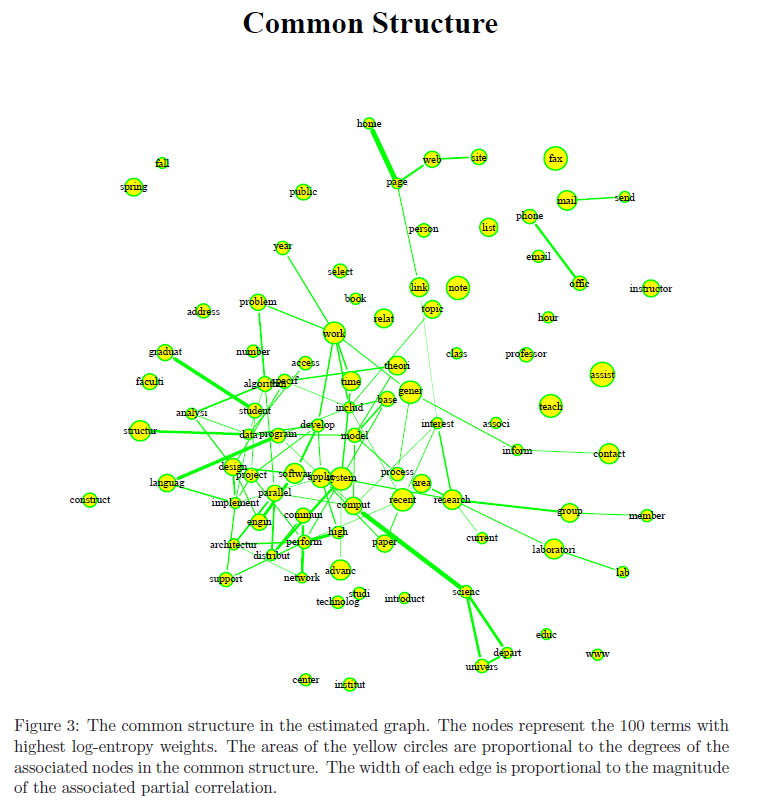
\includegraphics[height=3in]{guodata.png}
\end{frame}

\begin{frame}
\frametitle{Data Example}
\centering
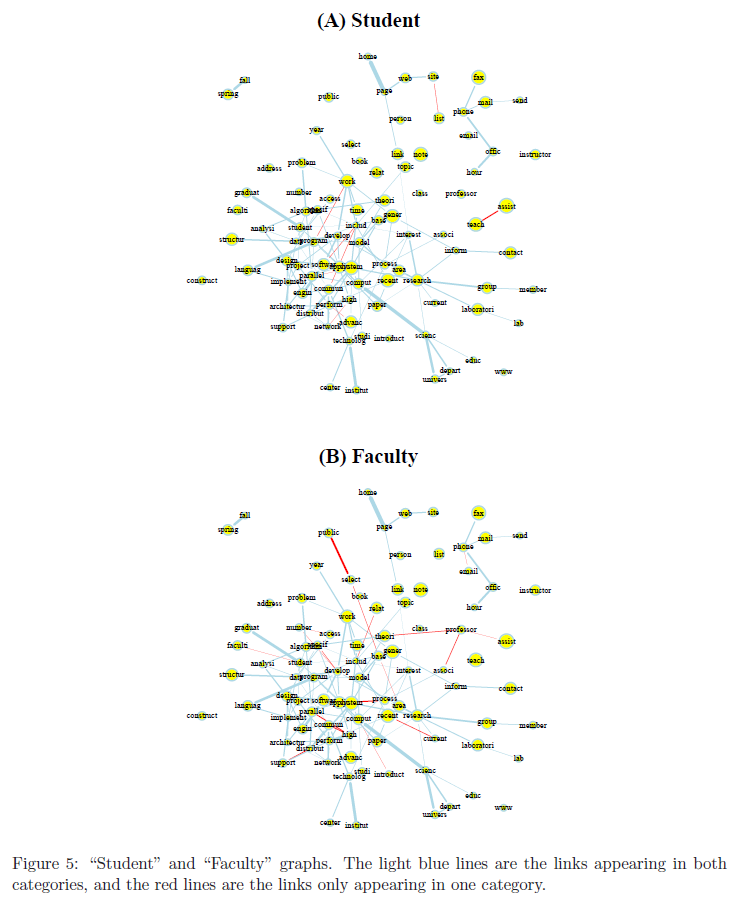
\includegraphics[height=3in]{guodata2.png}
\end{frame}


\begin{frame}
\frametitle{The Joint Graphical Lasso}
In their paper ``The joint graphical lasso for inverse covariance estimation across multiple classes,''  P. Danaher, P. Wang, \& D. Witten propose the \textit{joint graphical lasso} as a technique for jointly estimating multiple graphical models corresponding to distinct but related conditions, such as cancer and normal tissue.

\bigskip
\pause
Suppose we have data from $K \geq 2$ distinct classes.  Instead of estimating $\bm{\Sigma}_{1}^{-1},\bm{\Sigma}_{2}^{-1},\ldots,\bm{\Sigma}_{K}^{-1}$ separately, the authors propose estimating estimating these values jointly by maximizing the following penalized log-likelihood function
\small
\begin{equation*}
\max_{\{\bm{\Theta}\}} \sum_{k=1}^{K}n_{k}\left[\log\,\det \bm{\Theta}^{(k)}-\mbox{trace}\left(\bm{S}^{(k)}\bm{\Theta}^{(k)}\right)\right] - P(\{\bm{\Theta}\}),
\end{equation*}
\normalsize
subject to the constraint that $\bm{\Theta}^{(1)},\bm{\Theta}^{(2)},\ldots,\bm{\Theta}^{(K)}$ are positive definite, where $\{\bm{\Theta}\} = \{\bm{\Theta}^{(1)},\bm{\Theta}^{(2)},\ldots,\bm{\Theta}^{(K)}\}$.

\bigskip
\pause
$P(\{\bm{\Theta}\})$ denotes a convex penalty function, so the objective function is strictly concave.
\end{frame}

\begin{frame}
\frametitle{Joint Graphical Lasso}
Danaher et al.  propose choosing a penalty function $P$ that will encourage $\hat{\bm{\Theta}}^{(1)},\hat{\bm{\Theta}}^{(2)},\ldots,\hat{\bm{\Theta}}^{(K)}$ to share certain characteristics, such as the locations or values of the nonzero elements, in addition to providing sparse estimates of the precision matrices.

\bigskip
\pause
Two penalty functions suggested by Danaher et al. are the \textit{fused graphical lasso} and \textit{group graphical lasso} penalties.
\end{frame}

\begin{frame}
\frametitle{Fused Graphical Lasso}
The fused graphical lasso (FGL) penalty is given by
\small
\begin{equation*}
P(\{\bm{\Theta}\}) = \lambda_{1}\sum_{k=1}^{K}\sum_{i\neq j}|\theta_{ij}^{(k)}| + \lambda_{2}\sum_{k<k'}\sum_{i,j}|\theta_{ij}^{(k)}-\theta_{ij}^{(k')}|,
\end{equation*}
\normalsize
where $\lambda_{1}$ and $\lambda_{2}$ are nonnegative tuning parameters.

\bigskip
\pause
\begin{itemize}
	\item[1.] Like the graphical lasso, FGL results in sparse estimates $\hat{\bm{\Theta}}^{(1)},\hat{\bm{\Theta}}^{(2)},\ldots,\hat{\bm{\Theta}}^{(K)}$ when the tuning parameter $\lambda_{1}$ is large.
	
	\bigskip
	\pause
	\item[2.] Many of the elements $\hat{\bm{\Theta}}^{(1)},\hat{\bm{\Theta}}^{(2)},\ldots,\hat{\bm{\Theta}}^{(K)}$ will be identical across classes when the tuning parameter $\lambda_{2}$ is large.
	
	\bigskip
	\pause
	\item[3.] FGL borrows information aggressively across classes, encouraging not only similar network structure but also similar edge values.
\end{itemize}
\end{frame}

\begin{frame}
\frametitle{Group Graphical Lasso}
The group graphical lasso (GGL) penalty function is given by
\small
\begin{equation*}
P(\{\bm{\Theta}\}) = \lambda_{1}\sum_{k=1}^{K}\sum_{i\neq j}|\theta_{ij}^{(k)}| + \lambda_{2}\sum_{i\neq j}\sqrt{\sum_{k=1}^{K}\theta_{ij}^{(k)^{2}}},
\end{equation*}
\normalsize
where $\lambda_{1}$ and $\lambda_{2}$ are nonnegative tuning parameters.

\bigskip
\pause
\begin{itemize}
	\item[1.] The group lasso penalty encourages a similar pattern of sparsity across all of the precision matrices - there will be a tendency for the zeros in the $K$ estimated precision matrices to occur in the same places.
	
	\bigskip
	\pause
	\item[2.] When $\lambda_{1} = 0$ and $\lambda_{2} > 0$, each $\hat{\bm{\Theta}}^{(k)}$ will have an identical pattern of non-zero elements. On the other hand, the lasso penalty encourages further sparsity within each $\hat{\bm{\Theta}}^{(k)}$.
	
	\bigskip
	\pause
	\item[3.] GGL encourages a weaker form of similarity across the $K$ precision matrices than FGL in that GGL only encourages a shared pattern of sparsity and not shared edge values.
	\end{itemize}
\end{frame}

\begin{frame}
\frametitle{Algorithm for the Joint Graphical Lasso}
Danaher et al. solve the joint graphical lasso problem using an \textit{alternating directions method of multipliers} (ADMM) algorithm.

\bigskip
\pause
The original problem can be rewritten as
\small
\begin{equation*}
\min_{\{\bm{\Theta}\},\{\bm{Z}\}} -\sum_{k=1}^{K}n_{k}\left[\log\,\det \bm{\Theta}^{(k)}-\mbox{trace}\left(\bm{S}^{(k)}\bm{\Theta}^{(k)}\right)\right] + P(\{\bm{Z}\})
\end{equation*}
\normalsize
subject to the positive-definiteness constraint as well as the constraint that $\bm{Z}^{(k)} = \bm{\Theta}^{(k)}$, where $\{\bm{Z}\} = \{\bm{Z}^{(1)},\bm{Z}^{(2)},\ldots,\bm{Z}^{(k)}\}$.
\end{frame}


\begin{frame}
\frametitle{Algorithm for the Joint Graphical Lasso}
The scaled augmented Lagrangian for this problem is given by
\footnotesize
\begin{align*}
L_{\rho}(\{\bm{\Theta}\},\{\bm{Z}\},\{\bm{U}\}) =  -&\sum_{k=1}^{K}n_{k}\left[\log\,\det \bm{\Theta}^{(k)}-\mbox{trace}\left(\bm{S}^{(k)}\bm{\Theta}^{(k)}\right)\right] + P(\{\bm{Z}\}) \\
&+ \frac{\rho}{2}\sum_{k=1}^{K}||\bm{\Theta}^{(k)}-\bm{Z}^{(k)} + \bm{U}^{(k)}||_{F}^{2},
\end{align*}
\normalsize
where $\{\bm{U}\} = \{\bm{U}^{(1)},\bm{U}^{(2)},\ldots,\bm{U}^{(k)}\}$.

\bigskip
\pause
The ADMM corresponding to the above problem results in iterating three simple steps. 
\begin{itemize}
	\item[(a)] $\{\bm{\Theta}_{(i)}\} \leftarrow \mbox{arg\,min}_{\{\bm{\Theta}\}}\{L_{\rho}(\{\bm{\Theta}\},\{\bm{Z}_{(i-1)}\},\{\bm{U}_{(i-1)}\})\}$
	
	\smallskip
	\item[(b)] $\{\bm{Z}_{(i)}\} \leftarrow \mbox{arg\,min}_{\{\bm{Z}\}}\{L_{\rho}(\{\bm{\Theta}_{(i)}\},\{\bm{Z}\},\{\bm{U}_{(i-1)}\})\}$
	
	\smallskip
	\item[(c)] $\{\bm{U}_{(i)}\} \leftarrow \{\bm{U}_{(i-1)}\} + (\{\bm{\Theta}_{(i)}\} - \{\bm{Z}_{(i)}\})$.	
\end{itemize}

\bigskip
\pause
The update in step (a) preserves positive-definiteness, thus this constraint can be satisfied simply by initializing $\bm{\Theta}^{(k)}_{(0)} = \bm{I}$.

\end{frame}

\begin{frame}
\frametitle{Simulation Study}
The data for main simulation study consisted of 
generating three networks with p = 500 features belonging to ten
equally sized unconnected subnetworks, each with a power law degree
distribution, i.e. a scale-free network. Of the ten subnetworks, eight
have the same structure and edge values in all three classes, one is
identical between the first two classes and missing in the third
(i.e. the corresponding features are singletons in the third network),
and one is present in only the first class. The corresponding graph is shown in Figure \ref{graph1}. 

\smallskip
\pause

In addition to the 500-feature network pair, we generate a pair of
networks with p = 1000 features, each of which is block diagonal with
$500 \times 500$ blocks corresponding to two copies of the 500-feature
networks just described.
\end{frame}


\begin{frame}
\frametitle{Figure \ref{graph1}}
\begin{figure}
\centering 
                \includegraphics[scale=0.8]{{graph1danaher.pdf}}
                \caption{This shows the graph corresponding to the concentration matrix for the main simulation study. Black edges are common to all three classes, green edges are present only in classes 1 and 2, and red edges are present only in class 1.}
                \label{graph1}
\end{figure}
\end{frame}

\begin{frame}
\frametitle{Basic Result}
As we will see in the next slides, when $p = 500$ and $n= 150$, FGL performs the best in the simulations conducted by Danaher et. al. although it is much slower than $glasso$ (the fastest) and the group lasso penalty case. The graphical lasso and the joint estimation method introduced by Guo et al. (2011)  are included in the comparisons as well. 
\bigskip
\pause

In addition, FGL also seems to do better than GGL asymptotically when we hold $p$ to be fixed and let $n$ increase.
\end{frame}
\begin{frame}
\frametitle{In terms of parameters:}

FGL is presented in terms of $\lambda_2$
but for GGL they reparametrize the results in terms $\omega_2 = \frac{1}{\sqrt{2}}\lambda_2/(
\lambda_1 + \frac{1}{\sqrt{2}}\lambda_2)$. Each line corresponds to a different value of $\lambda_2$ and $\omega_2$.
\smallskip
\pause

As $\lambda_1$ or $\omega_1=\lambda_1 + \frac{1}{\sqrt{2}}\lambda_2$ increases, sparsity increases, or equivalently, the number of edges selected decreases.
\smallskip
\pause

According to the authors, approaches such as AIC, BIC, and cross-validation tend to choose models too large to be useful. In this setting, model selection should be guided by practical considerations, such as network interpretability, stability, and the desire for an edge set with a low false discovery rate.
\end{frame}

\begin{frame}
\frametitle{Some measures of error}

\begin{align*}
SSE = \sum_{k=1}^K \sum_{i \not= j} (\hat{\theta}^{(k)}_{ij} - (\Sigma^{(k)})^{-1}_{ij})^2
\end{align*}
\bigskip
\pause

Differential edges are defined as the edges that differ between classes. For FGL, it is computed
as the number of pairs $k<k',i<j$ such that $\hat{\theta}^{(k)}_{ij}
\not= \hat{\theta}^{(k')}_{ij}$. For GGL, the proposal of Guo et al. (2011), and the graphical lasso
it is computed as the number of pairs $k<k',i<j$ such
that $\abs{\hat{\theta}^{(k)}_{ij}- \hat{\theta}^{(k')}_{ij}} >
10^{-2}$.
\bigskip
\pause

The Kullback-Leibler Divergence (dKL) from the multivariate normal model with inverse covariance estimates $\Theta^{(1)},...,\Theta^{(k)}$to the multivariate
normal model with the true precision matrices $\Sigma^{(1)},...,\Sigma^{(k)}$
is 
\begin{align*}
\frac{1}{2} \sum_{k=1}^K (-\log \text{det} (\Theta^{(k)}\Sigma^{(k)}) + \text{trace}(\Theta^{(k)}\Sigma^{(k)}))
\end{align*}

\end{frame}

\begin{frame}
\frametitle{Figure 2 from Danaher et. al}
\begin{figure}
\centering 
                \includegraphics[width=\textwidth]{{Fig2Danimages.pdf}}
\end{figure}
\end{frame}

\begin{frame}
\frametitle{Figure 3 from Danaher et. al - Analysis of lung cancer microarray data}
\begin{figure}
\centering 
                \includegraphics[scale=0.8]{{Fig3Danaher.pdf}}
                \caption{Conditional dependency networks inferred from 17,772 genes in normal and cancerous lung cells. 278 genes have nonzero edges in at least one of the two networks. Black lines denote edges common to both classes. Red and green lines denote tumor-specific and normal-specific edges, respectively. The parameters used were $\lambda_1=0.95$ and $\lambda_2=0.005$.}
                \label{}
\end{figure}
\end{frame}

\begin{frame}
\frametitle{Table 1 from Danaher et. al}
\begin{figure}
\centering 
                \includegraphics[width=\textwidth]{{Table1Danaher.pdf}}
\end{figure}
\end{frame}

\begin{frame}
\frametitle{Table 1 indicates that}
for fixed $p$, as $n$ increases, FGL seems to do much better in terms of edge detection (as expected, sensitivity increases and false discovery rate decreases as $n$ increases) and differential edge detection (false discovery rate decreases as $n$ increases) than GGL. Oddly enough, in all cases, DED Sens declines as $n$ increases . 
\end{frame}

\begin{frame}
\frametitle{Nearest Neighbor Network (n = 100, p =25)}
\begin{table}
\begin{center}
\begin{tabular}{r|c|c}
\toprule
&\multicolumn{2}{c}{Group}\\
&$\lambda_1 = 0.07,\lambda_2 = 0.05$&$\lambda_1 = 0.05,\lambda_2 = 0.25$\\
\midrule
$F$&0.05642315&0.06010037\\  
$FP$&0.3391197&0.02918924\\   
$FN$&0.3035487&0.8517427\\         
\bottomrule
\end{tabular}
\caption[]{Nearest Neighbor Network for Group Lasso Penalty}
\label{tab:compare1}
\end{center}
\end{table}

\begin{table}
\begin{center}
\begin{tabular}{r|c|c}
\toprule
&\multicolumn{2}{c}{Fused}\\
&$\lambda_1 = 0.05,\lambda_2 = 0.05$&$\lambda_1 = 0.2,\lambda_2 = 0.1$\\
\midrule
$F$&0.06335103&0.06954624\\  
$FP$&0.4269327&0.002245857\\   
$FN$&0.3139659&0.9723261\\         
\bottomrule
\end{tabular}
\caption[]{Nearest Neighbor Network for Fused Lasso Penalty}
\label{tab:compare2}
\end{center}
\end{table}
\end{frame}

\begin{frame}
\frametitle{$\hat{\Omega}_1$ for Nearest Neighbor Network (n = 100, p =25)}
\begin{figure}
\centering 
\begin{subfigure}[b]{0.40\textwidth}
  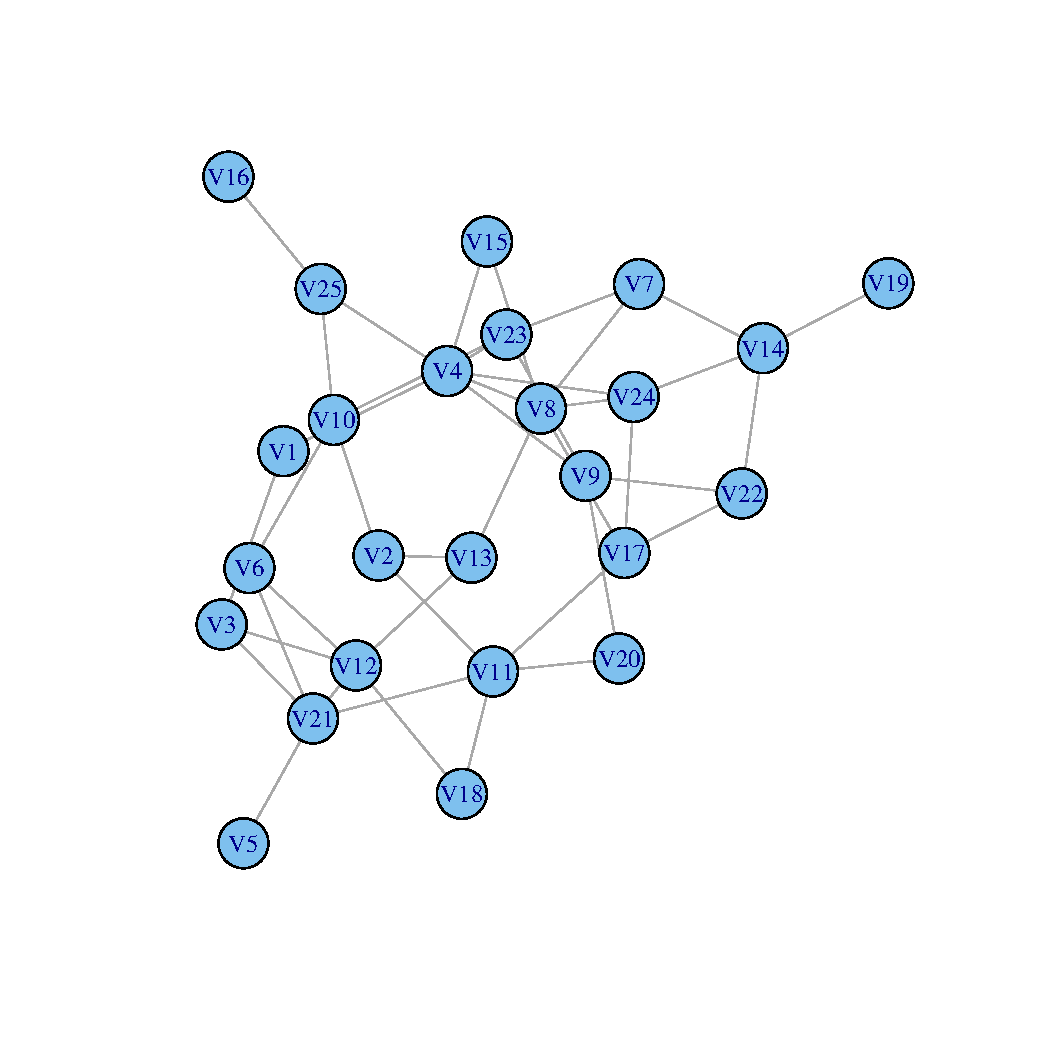
\includegraphics[scale=0.15]{Omega1hat-f.pdf}
  \caption{Estimated Nearest Neighbor Graph with Fused Lasso Penalty}
\label{fig:nearestgaphsestimate}
\end{subfigure}
\begin{subfigure}[b]{0.40\textwidth}
  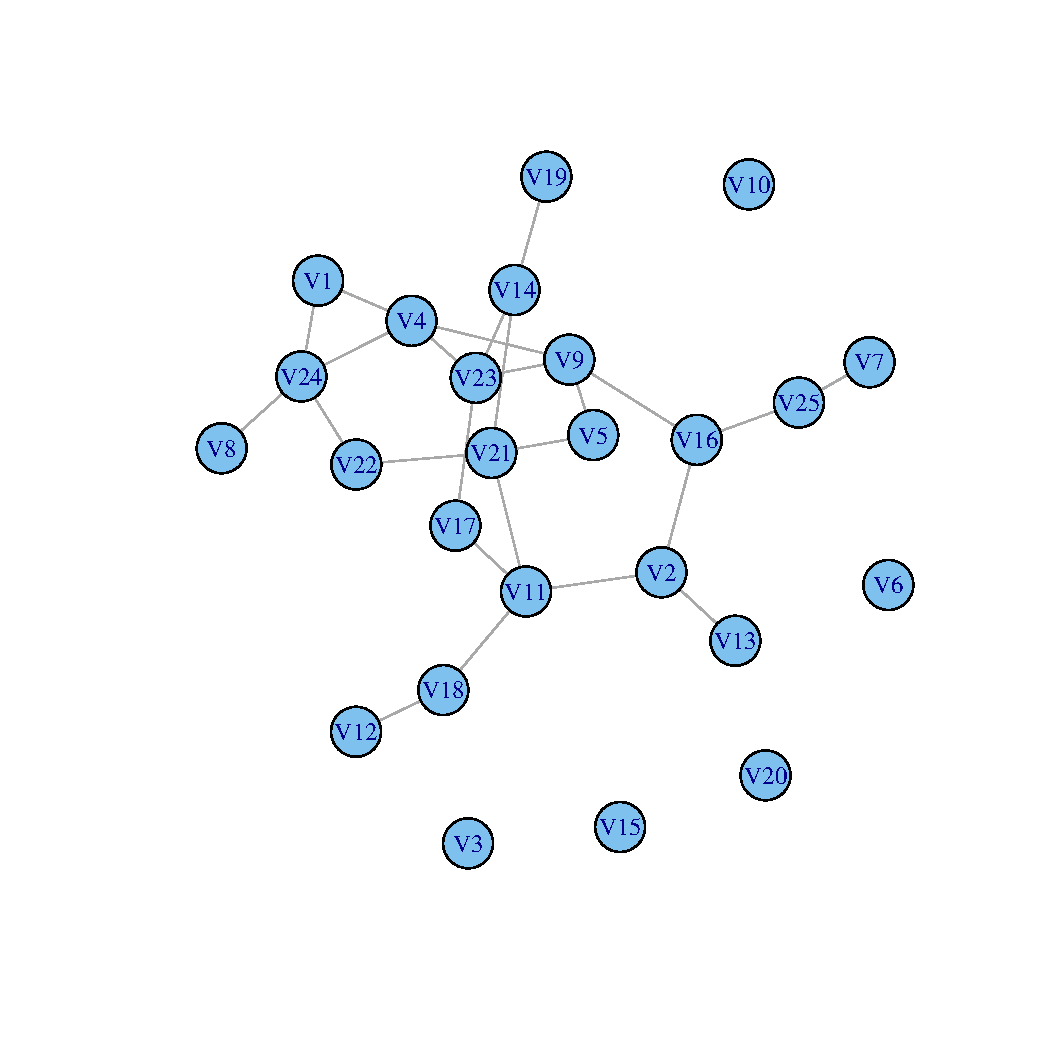
\includegraphics[scale=0.15]{Omega1hat-g.pdf}
  \caption{Estimated Nearest Neighbor Graph with Group Lasso Penalty}
\label{fig:nearestgaphsestimate}
\end{subfigure}\\
\begin{subfigure}[b]{0.50\textwidth}
  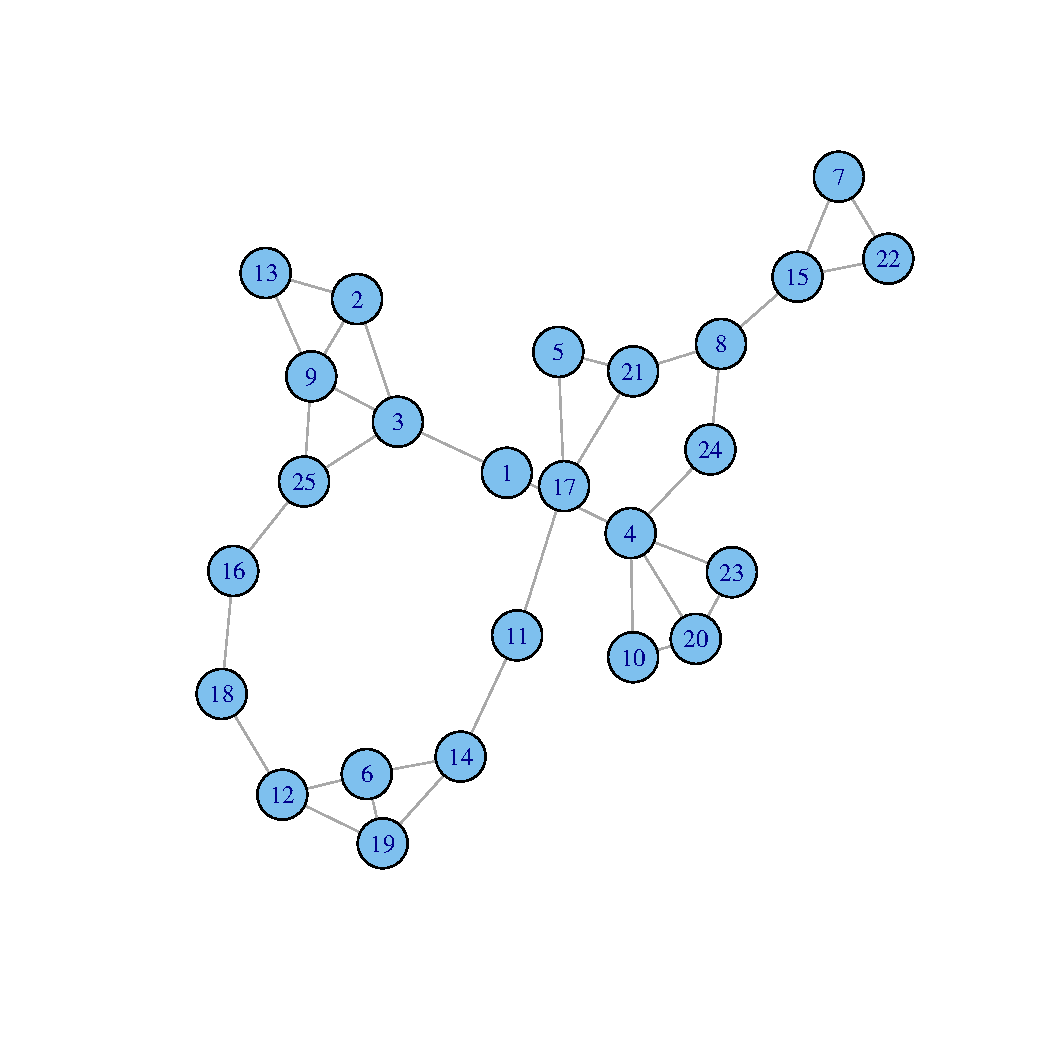
\includegraphics [scale=0.15]{Omega1-f.pdf}
  \caption{True Nearest Neighbor Graph}
\label{fig:nearestgaphsactual}
\end{subfigure}
\end{figure}
\end{frame}

\begin{frame}
\frametitle{$\hat{\Omega}_2$ for Nearest Neighbor Network (n = 100, p =25)}
\begin{figure}
\centering 
\begin{subfigure}[b]{0.40\textwidth}
  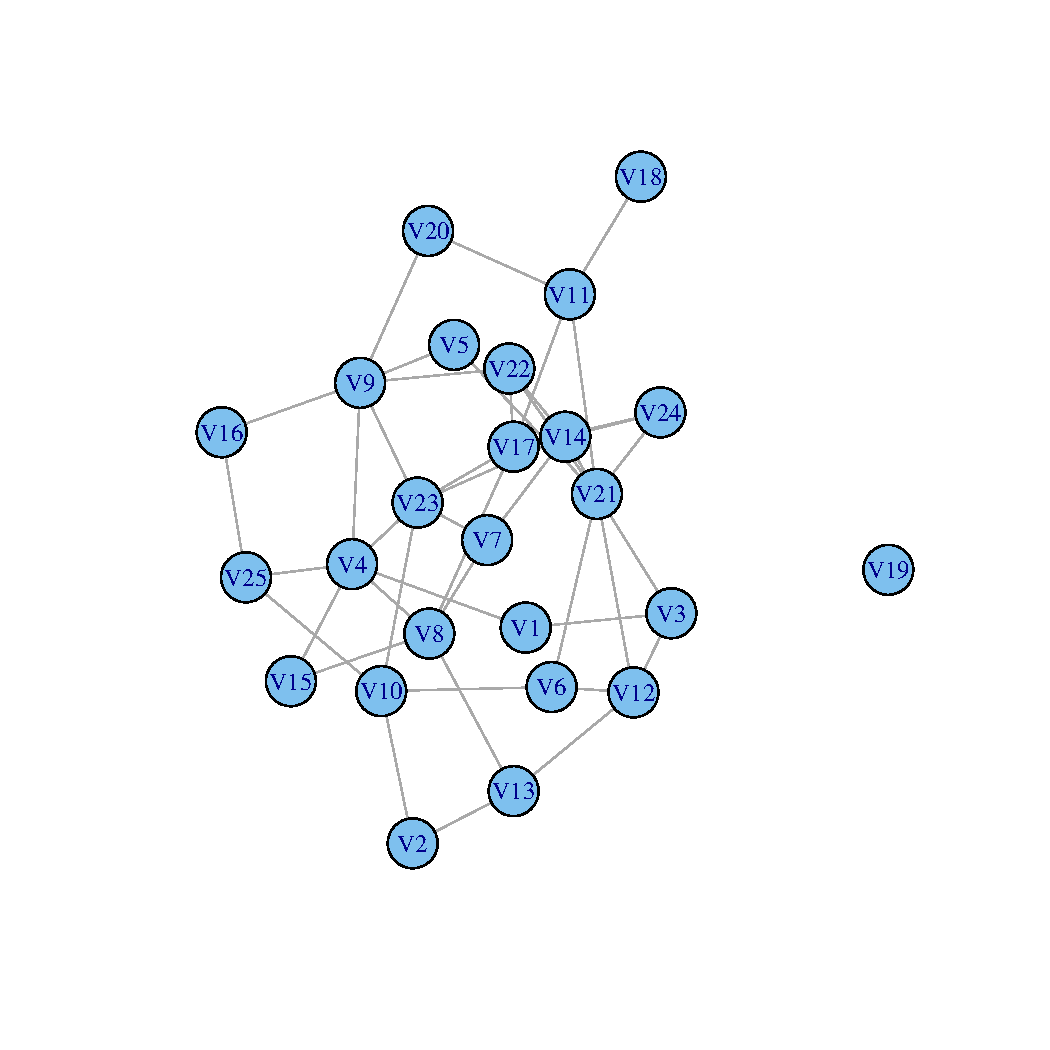
\includegraphics[scale=0.15]{Omega2hat-f.pdf}
  \caption{Estimated Nearest Neighbor Graph with Fused Lasso Penalty}
\label{fig:nearestgaphsestimate}
\end{subfigure}
\begin{subfigure}[b]{0.40\textwidth}
  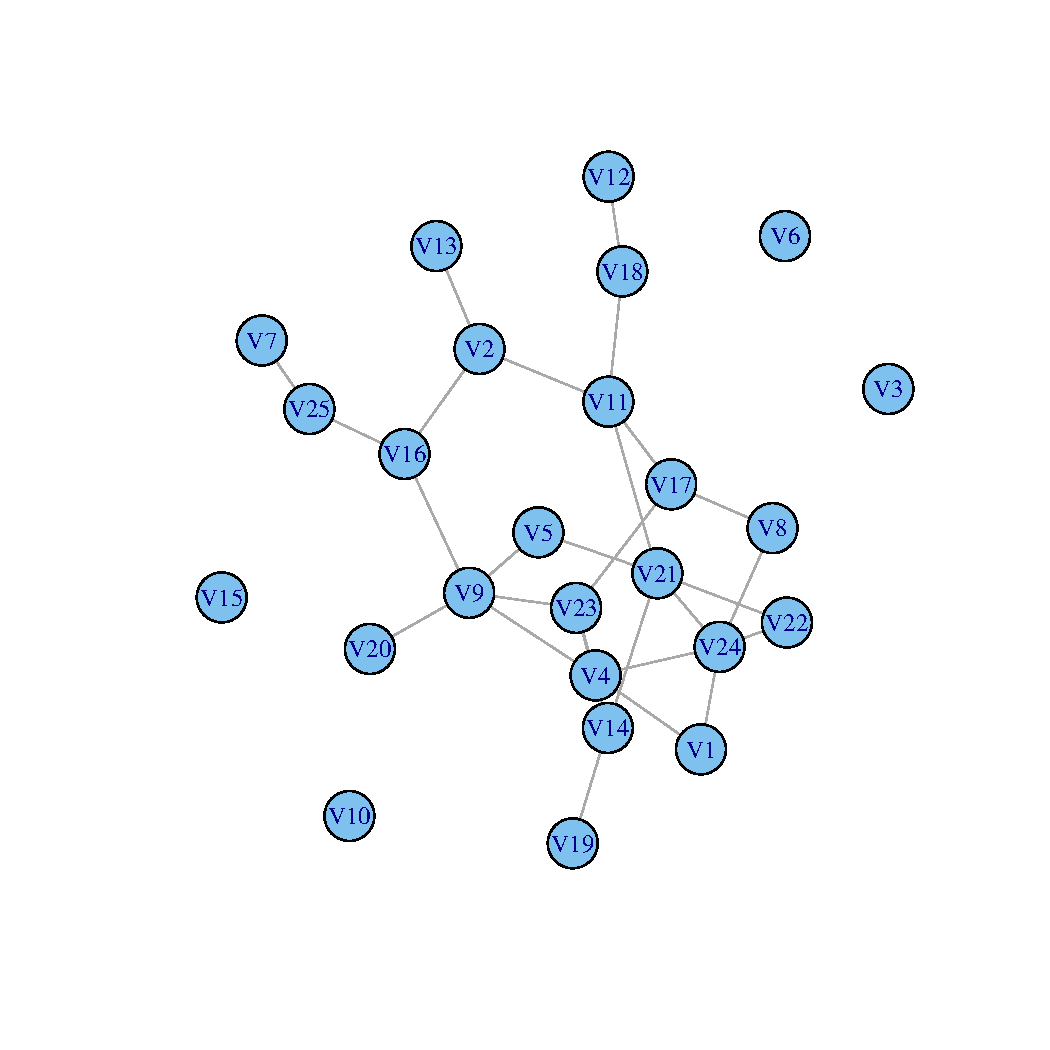
\includegraphics[scale=0.15]{Omega2hat-g.pdf}
  \caption{Estimated Nearest Neighbor Graph with Group Lasso Penalty}
\label{fig:nearestgaphsestimate}
\end{subfigure}\\
\begin{subfigure}[b]{0.50\textwidth}
  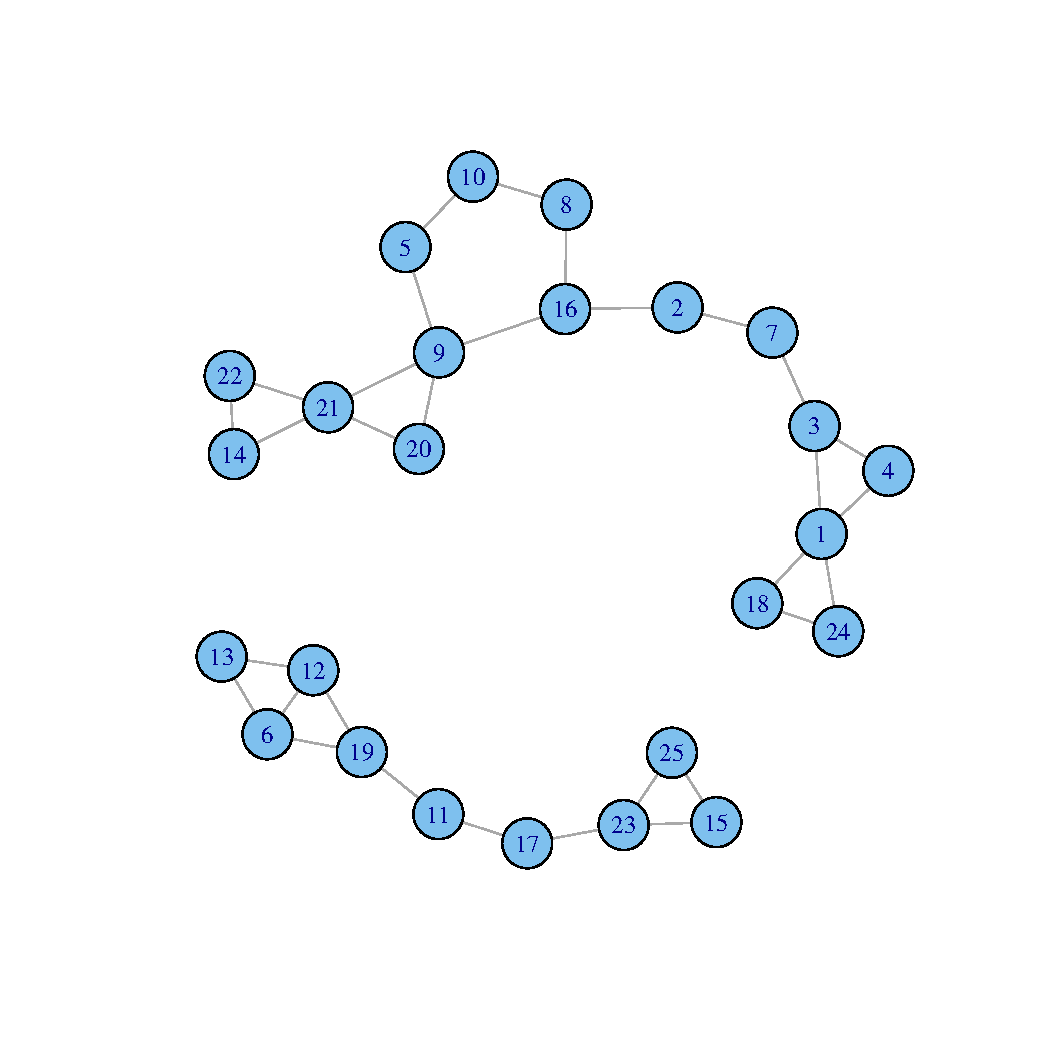
\includegraphics [scale=0.15]{Omega2-f.pdf}
  \caption{True Nearest Neighbor Graph}
\label{fig:nearestgaphsactual}
\end{subfigure}
\end{figure}
\end{frame}

\begin{frame}
\frametitle{$\hat{\Omega}_3$ for Nearest Neighbor Network (n = 100, p =25)}
\begin{figure}
\centering 
\begin{subfigure}[b]{0.40\textwidth}
  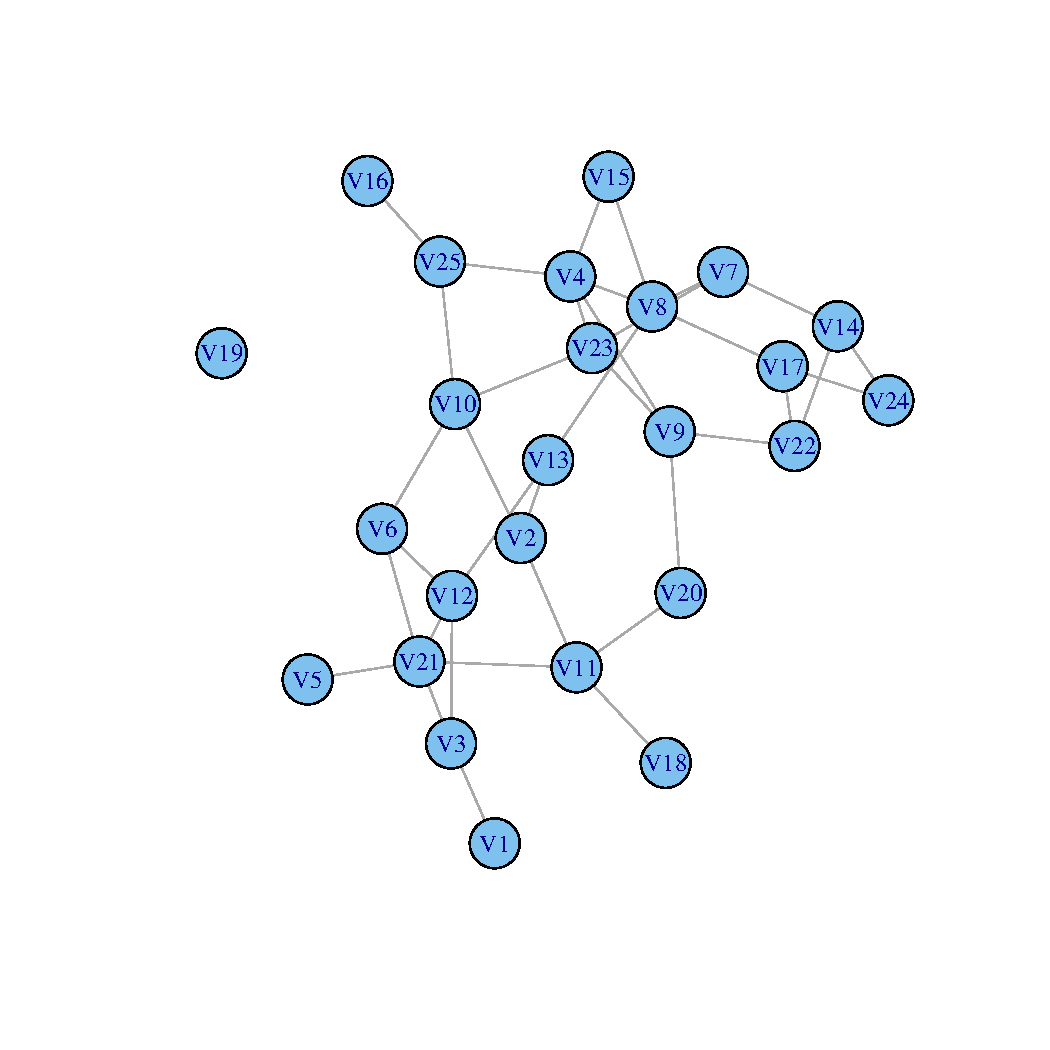
\includegraphics[scale=0.15]{Omega3hat-f.pdf}
  \caption{Estimated Nearest Neighbor Graph with Fused Lasso Penalty}
\label{fig:nearestgaphsestimate}
\end{subfigure}
\begin{subfigure}[b]{0.40\textwidth}
  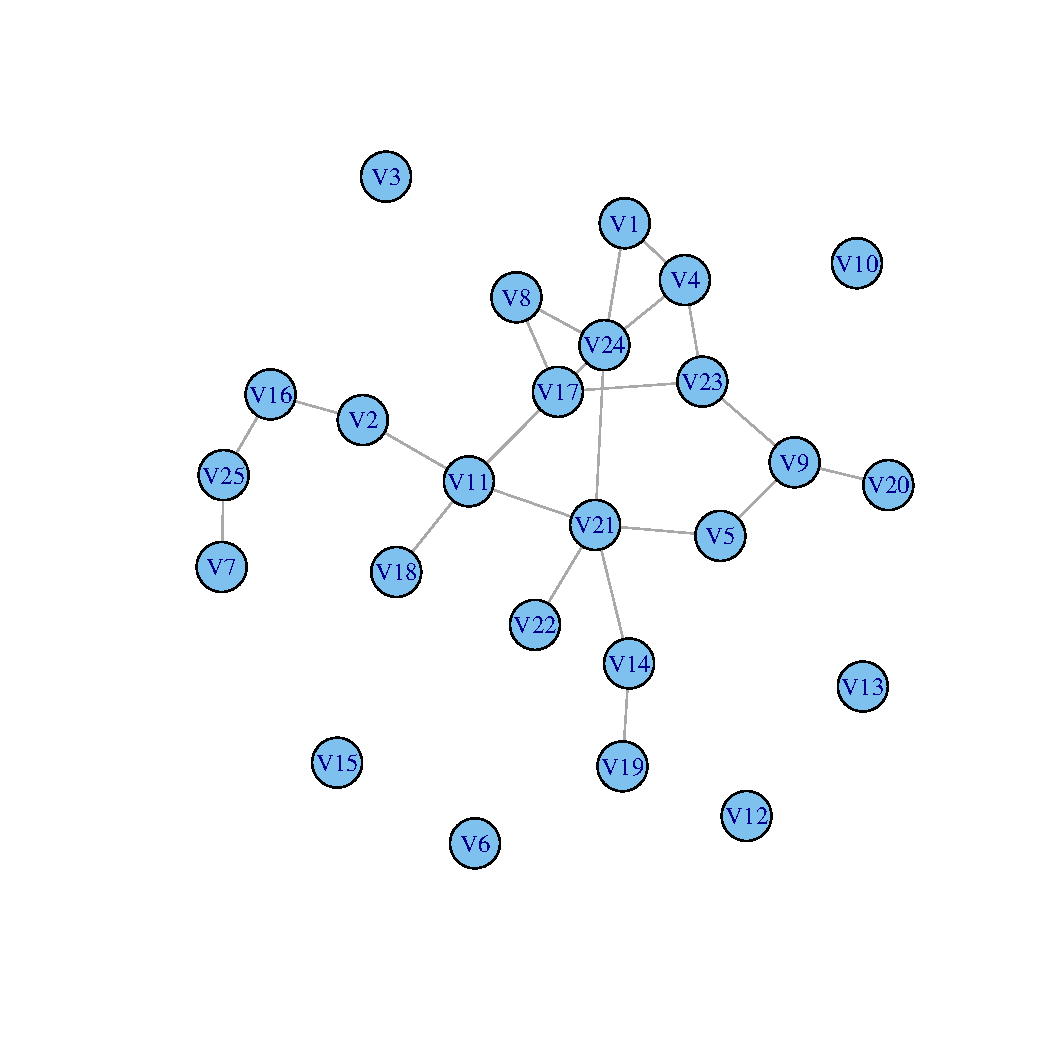
\includegraphics[scale=0.15]{Omega3hat-g.pdf}
  \caption{Estimated Nearest Neighbor Graph with Group Lasso Penalty}
\label{fig:nearestgaphsestimate}
\end{subfigure}\\
\begin{subfigure}[b]{0.50\textwidth}
  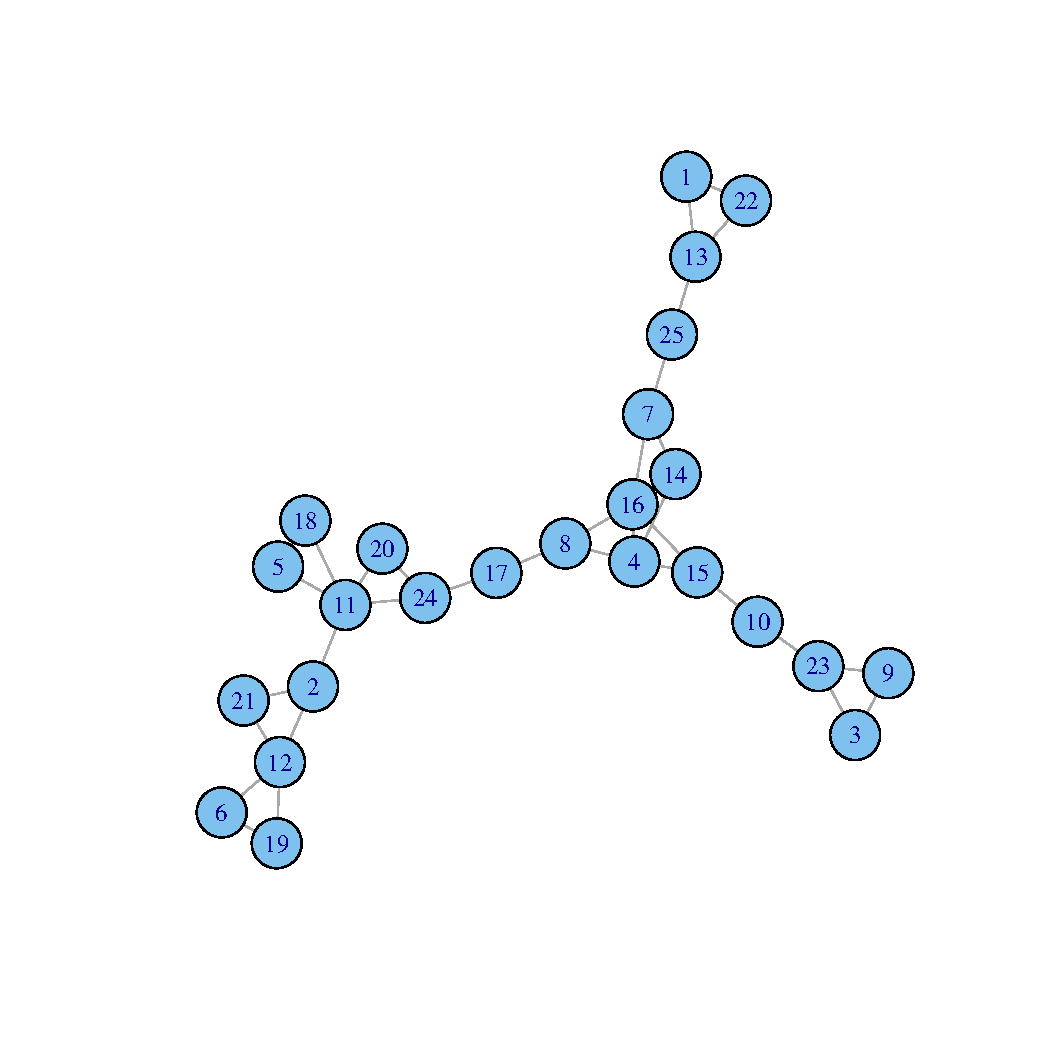
\includegraphics [scale=0.15]{Omega3-f.pdf}
  \caption{True Nearest Neighbor Graph}
\label{fig:nearestgaphsactual}
\end{subfigure}
\end{figure}
\end{frame}

\begin{frame}
\frametitle{Additional notes}
In the appendix, they show that if you go down to 2 classes, FGL performs as fast as GGL while still maintaining the results best overall.

\bigskip
\pause
We thought it was odd that the authors were much more interested in having  a low false positive rate at the cost of a high false negative instead of a balance between the two. 

\bigskip
\pause
Danaher et al. claim that FGL and GGL are superior to existing methods such as time-varying networks (FGL and GGL do not require a natural ordering) and Guo et al. (penalty in Guo et.al lacks convexity, uses only one tuning parameter). In addition, FGL is superior to other methods when we expect edge values as well as network structure to be similar across classes. 

\end{frame}

%\bibliographystyle{ims}
%\nocite{*}

%\begin{frame}[allowframebreaks]
%\tiny
%        \frametitle{References}
%        \bibliographystyle{amsalpha}
%        %\bibliography{../bib_files/jabrefmaster.bib}
%        \bibliography{references}
%\end{frame}
%



\end{document}

